\subsection{Konceptarkitektur}
Konceptarkitekturen ger en översikt över arkitekturen för hela systemet. Den illustrerar uppdelningen i de mest centrala komponenterna och deras ansvarsområden. De huvudsakliga datavägarna och vilken data som flödar genom dem åskådliggörs också.

\subsubsection{Modell}
Modellen i figur \ref{fig:konceptarkitektur} beskriver konceptarkitekturen. Streckade linjer representerar i detta fall nätverkskommunikation. Vid de båda komponenterna som benämns med GUI finns förtydlingar över att dessa är användargränssnitt och färmed uppfyller stereotypen \textit{Presentation} \cite[p.~50--51]{bib-architecture-primer}. Use case maps för denna arkitektur återfinns i appendix \ref{sec:use_case_koncept}.

\begin{figure}[h]
    \centering
    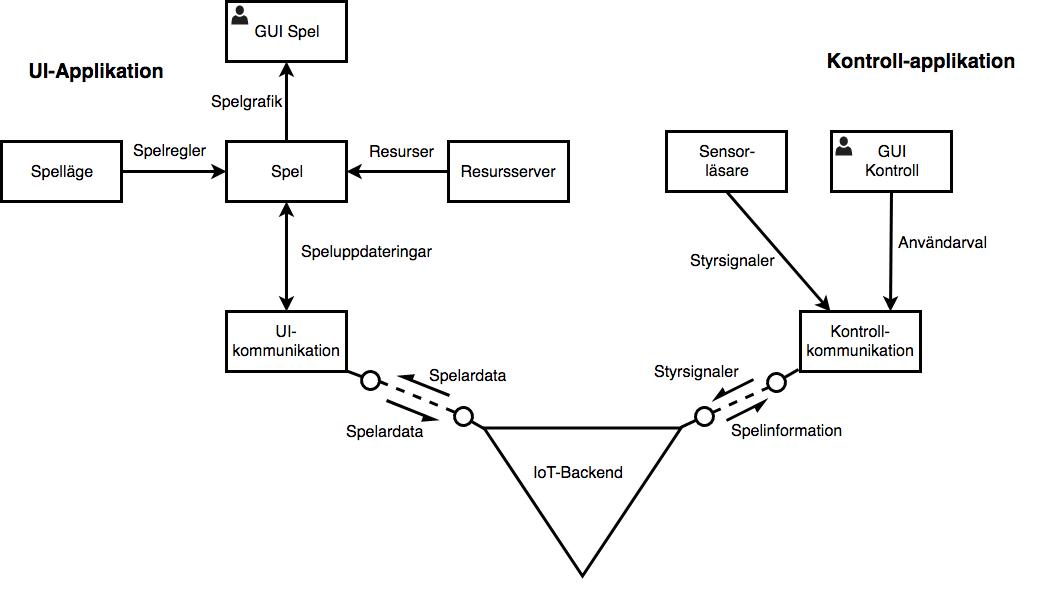
\includegraphics[scale=0.4]{konceptarkitektur}
    \caption{Modell över konceptarkitektur}
    \label{fig:konceptarkitektur}
\end{figure}

\subsubsection{Ansvarsområden}
\begin{labeling}{\small{\textbf{Kontrollkommunikation}}}
    \item [\small{\textbf{GUI Spel}}]
        \begin{itemize}
            \item Visa upp spelplanen
            \item Visa upp menyer
            \item Starta spel med specifika inställningar
            \newline
        \end{itemize}

    \item [\small{\textbf{Spelläge}}]
        \begin{itemize}
            \item Sätta upp regler för spelet
            \item Avgöra vilka resurser spelet ska innehålla
            \item Avgöra vad som ska ske vid olika tillfällen i spelet
            \newline
        \end{itemize}

    \item [\small{\textbf{Spel}}]
        \begin{itemize}
            \item Hålla koll på de olika spelarna
            \item Tillhandahålla grundläggande spelmekanik
            \newline
        \end{itemize}

    \item [\small{\textbf{Resursserver}}]
        \begin{itemize}
            \item Lagra vilka resurser som finns
            \item Ladda in resurser
            \newline
        \end{itemize}

    \item [\small{\textbf{UI-kommunikation}}]
        \begin{itemize}
            \item Upprätta uppkoppling mot server
            \item Förpacka data för kommunikation
            \newline
        \end{itemize}

    \item [\small{\textbf{Sensorläsare}}]
        \begin{itemize}
            \item Läsa av data från sensor
            \item Abstrahera sensordata till standardiserad form
            \item konfigurera sensor
            \newline
        \end{itemize}

    \item [\small{\textbf{GUI-kontroll}}]
        \begin{itemize}
            \item Visa menyer för att gå med i spelinstans
            \item Visa spelinformation om pågående spelet
            \item Tillhandahålla knappar på skärmen
            \newline
        \end{itemize}

    \item [\small{\textbf{Kontrollkommunikation}}]
        \begin{itemize}
            \item Upprätta uppkoppling mot server
            \item Förpacka data för kommunikation
            \newline
        \end{itemize}

    \item [\small{\textbf{IoT-Backend}}]
        \begin{itemize}
            \item Dirigera data mellan olika Kontroll-applikationer och olika instanser av UI-applikationen.
            \item Verifiera koder för att gå med i specifika spelinstanser.
            \newline
        \end{itemize}
\end{labeling}

\subsubsection{Beskrivning}
Arkitekturen är tydligt uppdelad i UI-applikation och kontroll-applikation. Från båda dessa finns specifika enheter som hanterar kommunikationen med den IoT-backend som är central i systemet. Dessa komponenters roll är att erbjuda ett gemensamt gränssnitt utåt för dataflöde. Då dessa två komponenter till stor del innehåller samma funktionalitet bör även delar av implementationen kunna återanvändas.\\

De två resursservrarna ska ses som instanser av samma komponent. Implementationen för dessa ska göras så pass generell att den kan användas både på UI- och kontroll-applikationen. En resursservers uppgift är att flytta ut arbetet med att ladda in resurser från implementationen i andra komponenter. I denna komponent finns också stora möjligheter att använda sig av cachning för Progressive Web Apps (referens?).\\

Spelläget är i denna modell en ensam komponent med endast ett gränssnitt mot den grundläggande spellogiken. Detta gränssnitt ska vara väldefinierat för att underlätta skapandet av nya spellägen. Med den nära kopplingen till resten av spelet finns också bra möjligheter till många kreativa spellägen, utan begränsing av omgivningen i systemet.\\

I arkitekturen för mobil-applikationen finns endast några få komponenter som uppfyller de nödvändiga kraven. Hela denna applikation får i denna struktur främst som uppgift att läsa data och skicka denna vidare. Detta är en lätt, icke prestandakrävande struktur.\\

Då arkitekturen inte består av många lager hålls datavägar genom den korta. Detta är centralt för responsivitet i en realtidsapplikation. Speciellt värt att notera är hur sensordata i kontroll-applikationen ej behöver passera fler komponenter för att nå applikationens kommunikations-gränssnitt.\\

Komponenten IoT-Backend är till viss del ett redan existerande system, men kommer att utökas med viss funktionalitet under projektet. I modellen är denna utökning ej separerad från resten av det systemet. Funktionalitet för att dirigera data kommer behöve skötas här för att tillåta flera olika instanser av UI-applikationen. Även all hantering av koder för anslutning till olika instanser bör därför implementeras i komponenten IoT-Backend.\\
